% ===== 第一部分：单变量分析学 / 第7章：微分法 =====
% !TEX root = ../../main.tex
\setchapterimage{figure/chapter7封面图.png}
\setchapterintro{这一章讲单变量函数的微分法，开篇证明微分与导数的等价性，建立起了可导与连续的关系，之后介绍了微分中值定理，Taylor公式等重要内容。}
\chapter{微分法}
% 第1节：导数、微分与连续性
% !TEX root = ../../../main.tex
% 所属：第一部分：单变量分析学 / 第7章：微分法
% 节：7.1 导数、微分与连续性
% 正文按原文件顺序保存；由 ../chapter7.tex 调用。
\section{导数、微分与连续性}
\begin{definition}
	$y=f(x)$ 在 $x_0$ 的某个邻域 $O\left(x_0, \rho\right)$ 上有定义，若 $\forall \Delta x\left(x_0+\Delta x \in O\left(x_0, \rho\right)\right)$ ，极限
	
	$$
	\lim _{\Delta x \rightarrow 0} \frac{f\left(x_0+\Delta x\right)-f\left(x_0\right)}{\Delta x}
	$$
	
	
	存在且有限，则称 $f(x)$ 在 $x=x_0$ 可导，该极限称为 $f(x)$ 在 $x=x_0$ 处的导数，记为 $f^{\prime}\left(x_0\right)$ .
	

\end{definition}	等价地，$f^{\prime}\left(x_0\right)$ 可以写作

$$
f^{\prime}\left(x_0\right)=\lim _{t \rightarrow x_0} \frac{f(t)-f\left(x_0\right)}{t-x_0}
$$


若 $f(x)$ 在 $(a, b)$ 上任一点处可导，则称 $f(x)$ 在 $(a, b)$ 上可导，记为$f\in D(a,b)$,若$f$的导函数也是连续的，则记为$f\in C^1(a,b)$
\begin{definition}
	$ y=f(x)$ 在 $O\left(x_0, \rho\right)$ 上有定义，$\forall \Delta x\left(x_0+\Delta x \in O\left(x_0, \rho\right)\right).$ 
	极限
	
	$$
	\lim _{\Delta x \rightarrow 0^{+}} \frac{f\left(x_0+\Delta x\right)-f\left(x_0\right)}{\Delta x}
	$$
	
	
	存在且有限，则称 $f(x)$ 在 $x=x_0$ 处右可导，记为 $f^{\prime}_{+}\left(x_0\right)$ ，称右导数.
	
	类似地，定义 $$f^{\prime}_{-}\left(x_0\right)=\lim _{\Delta x \rightarrow 0^{-}} \frac{f\left(x_0+\Delta x\right)-f\left(x_0\right)}{\Delta x}$$
	显然地，$f^{\prime}\left(x_0\right)$ 存在的充要条件是 $f_{+}^{\prime}\left(x_0\right)=f_{-}^{\prime}\left(x_0\right)=f\left(x_0\right)$
	
	若 $f^{\prime}_{+}\left(x_0\right) \neq f^{\prime}\left(x_0\right)$ ，或其中有不存在者，则称 $x_0$ 为 $f(x)$ 的不可导点
	
	与连续性类似的，我们可以给出一个函数在闭区间上可导的定义：$f\in D(a,b)$，且$f'_{+}(a),f'_{-}(b)$存在且有限
\end{definition}
\begin{definition}
	$y=f(x)$ 在 $x_0$ 的某个邻域 $O\left(x_0, \rho\right)$ 上有定义，若 $\Delta x \rightarrow 0$ 时，$$\quad \Delta y=f\left(x_0+\Delta x\right)-f\left(x_0\right)=A\left(x_0\right) \Delta x+o(\Delta x)$$则称 $y=f(x)$ 在 $x_0$ 处可微，记其微分为
	$$\mathrm{d} y|_{y=y_0}=A\left(x_0\right) \mathrm{d} x$$
\end{definition}
\begin{theorem}
	$y=f(x)$在$x=x_0$处可导的充要条件是$f(x)$在$x_0$处可微.
\end{theorem}
\begin{proof}
	必要性：已知 $f(x)$ 在 $x_0$ 处可导，由定义
	$$f^{\prime}\left(x_0\right)=\lim _{\Delta x \rightarrow 0} \frac{f\left(x_0+\Delta x\right)-f\left(x_0\right)}{\Delta x}$$
	存在一个函数 $\varphi(\Delta x) \rightarrow 0(\Delta x \rightarrow 0$ 时 $)$
	使得 $|\Delta x|$ 充分小时,
	$$\frac{f\left(x_0+\Delta x\right)-f\left(x_0\right)}{\Delta x}=f^{\prime}\left(x_0\right)+\varphi(\Delta x)$$那么$$\Delta y=f\left(x_0+\Delta x\right)-f\left(x_0\right)=f^{\prime}\left(x_0\right) \Delta x+\varphi(\Delta x) \Delta x=f^{\prime}\left(x_0\right) \Delta x+o(\Delta x)$$
	从而 $y=f(x)$ 在 $x=x_0$ 处可微且 $\mathrm{d}y =f^{\prime}(x) \mathrm{d} x$
	
	充分性：已知 $y=f(x)$ 在 $x=x_0$ 处可微，存在一个仅与 $x_0$ 有关的量 $A(x_0)$使得
	$$\begin{aligned}
		\Delta y=f\left(x_0+\Delta x\right)-f\left(x_0\right)=A\left(x_0\right) & \Delta x+o(\Delta x) \\
		\frac{\Delta y}{\Delta x}=\frac{f\left(x_0+\Delta x\right)-f\left(x_0\right)}{\Delta x} & =A\left(x_0\right)+\frac{o(\Delta x)}{\Delta x} \\
		& \rightarrow A\left(x_0\right)(\Delta x \rightarrow 0 \text { 时 })
	\end{aligned}$$
	$f(x)$ 在 $x=x_0$ 处可导，且 $A\left(x_0\right)=f^{\prime}\left(x_0\right)$ ，故有 $\mathrm{d} y=f^{\prime}(x) \mathrm{d} x$
	
	
\end{proof}
综上 $ f^{\prime}(x)=\dfrac{\mathrm{d} y}{\mathrm{d} x}$

对 $\mathbb{R}^{1}$ 上的函数，可导等价于可微.

对上式的两端,$f^{\prime}(x)$ 是一个整体,$\dfrac{\mathrm{d} y}{\mathrm{d} x}$ 又称微商,它可以做乘除的运算.
\begin{proposition}
	$y=f(x)$ 在 $x=x_0$ 处可导，则 $f(x)$ 在 $x=x_0$ 处连续.
\end{proposition}


\begin{proof}
	设 $f(x)$ 在 $x=x_0$ 处可导，$|\Delta x|$ 充分小时,$\exists \varphi(x) \rightarrow 0(x \rightarrow 0)$,使得$$f\left(x_0+\Delta x\right)-f\left(x_0\right)=f^{\prime}\left(x_0\right) \Delta x+\varphi(\Delta x)$$
	
	$\Delta x \rightarrow 0$ 时，上式右侧$\rightarrow 0$ ,故$$\lim _{\Delta x \rightarrow 0} f\left(x_0+\Delta x\right)=f\left(x_0\right)$$
	
	这就是连续性的定义.
\end{proof}
连续不一定可导，例如 $y=|x|$ 在 $x=0$ 处


%
% 第2节：导数的运算与法则
% !TEX root = ../../../main.tex
% 所属：第一部分：单变量分析学 / 第7章：微分法
% 节：7.2 导数的运算与法则
% 正文按原文件顺序保存；由 ../chapter7.tex 调用。
\section{导数的运算与法则}
\begin{proposition}\label{calofder}
	$f, g$ 定义在 $[a, b]$ 上，并且都在点 $x \in[a, b]$ 可导，那么 $f+g, f g, \dfrac{f}{g}$ 也在 $x$ 点可导，而且：
	
	（a）$$(f+g)^{\prime}(x)=f^{\prime}(x)+g^{\prime}(x)$$
	
	（b）$$\left(f g)^{\prime}(x)=f^{\prime}(x) g(x)+f(x) g^{\prime}(x)\right.$$
	
	（c）$$\left(\dfrac{f}{g}\right)^{\prime}(x)=\dfrac{g(x) f^{\prime}(x)-g^{\prime}(x) f(x)}{g^2(x)}$$
	
	对 $(c)$ ，假定 $g(x) \neq 0$
\end{proposition}

\begin{proof}
	(a) $$\begin{aligned} \lim _{\Delta x \rightarrow 0} \frac{(f+g)(x+\Delta x)-(f+g)(x)}{\Delta x} & =\lim _{\Delta x \rightarrow 0} \frac{f(x+\Delta x)-f(x)}{\Delta x}+\lim _{\Delta x \rightarrow 0} \frac{g(x+\Delta x)-g(x)}{\Delta x} \\ & =f^{\prime}(x)+g^{\prime}(x)\end{aligned}$$
	
	(b)令$h=fg$,则
	$$h(x+\Delta x)-h(x)=f(x+\Delta x)(g(x+\Delta x)-g(x))+g(x)(f(x+\Delta x)-f(x))$$
	带入得
	$$\begin{aligned} \lim _{\Delta x \rightarrow 0} \frac{(f g)(x+\Delta x)-(f g)(x)}{\Delta x} & =\lim _{\Delta x \rightarrow 0} f(x+\Delta x) \frac{g(x+\Delta x)-g(x)}{\Delta x}+g(x) \frac{f(x+\Delta x)-f(x)}{\Delta x} \\ & =f(x) g^{\prime}(x)+g(x) f^{\prime}(x)\end{aligned}$$
	
	(c)$$\begin{aligned}
		&\lim _{\Delta x \rightarrow 0} \dfrac{\left(\dfrac{f}{g}\right)(x+\Delta x)-\left(\dfrac{f}{g}\right)(x)}{\Delta x}\\ & =\lim _{\Delta x \rightarrow 0} \dfrac{1}{g(x) g(x+\Delta x)}\left[g(x) \dfrac{f(x+\Delta x)-f(x)}{\Delta x}-f(x) \dfrac{g(x+\Delta x)-g(x)}{\Delta x}\right] \\
		& =\dfrac{f^{\prime}(x) g(x)-f(x) g^{\prime}(x)}{g^2(x)}
	\end{aligned}$$
	
\end{proof}
上述定理的微分形式为

（a）$\mathrm{d}[f(x)+g(x)]=\mathrm{d}[f(x)]+\mathrm{d}[g(x)]$

（b）$\mathrm{d}[(f g)(x)]=\mathrm{d}[f(x)] g(x)+f(x) \mathrm{d}[g(x)]$

（c）$\mathrm{d}\left[\left(\dfrac{f}{g}\right)(x)\right]=\dfrac{\mathrm{d}[f(x)] g(x)-f(x) \mathrm{d}[g(x)]}{g^2(x)}$

更一般地，有 $$\left[\sum_{i=1}^n c_i f_i(x)\right]^{\prime}=\sum_{i=1}^n c_i f_i^{\prime}(x)$$

$$
\left[\prod_{i=1}^n f_i(x)\right]^{\prime}=\sum_{j=1}^n\left\{f_j^{\prime}(x) \prod_{i=1, i\neq j}^n f_i(x)\right\}
$$
\begin{theorem}(反函数求导定理)
	设 $y=f(x)$ 在 $(a, b)$ 上连续，严格单调，可导且 $f^{\prime}(x) \neq 0$ ，设
	
	$$
	\alpha=\min \left\{f(a+), f(b-)\right\}, \beta=\max\left\{f(a+), f(b-)\right\}  .
	$$
	
	
	则反函数 $x=f^{-1}(y)$ 在 $(\alpha, \beta)$ 上存在且
	
	$$
	\left(f^{-1}(y)\right)^{\prime}=\frac{1}{f^{\prime}(x)}=\frac{1}{f^{\prime}\left(f^{-1}(y)\right)}
	$$
\end{theorem}
1, $ \alpha$ 可以为 $-\infty, \beta$ 可以为 $+\infty $ 

2,若 $f^{\prime}\left(x_0\right)=0$ ，则 $(f^{-1}(y))^{\prime}=\dfrac{1}{f^{\prime}(x)}$ 在 $x_0$ 处不成立
\begin{proof}
	取 $\Delta y$ ,使得$y+\Delta y \in(\alpha, \beta)$ ，不妨设 $f$ 严格单调增加,$y=f(x), y+\Delta y=f(x+\Delta x)$ ,由 $x=f^{-1}(y)$ 的连续性, $\Delta y \rightarrow 0$ 时 $\Delta x \rightarrow 0$
	
	$$
	\frac{f^{-1}(y+\Delta y)-f^{-1}(y)}{\Delta y}=\frac{\Delta x}{f(x+\Delta x)-f(x)}=\left(\frac{f(x+\Delta x)-f(x)}{\Delta x}\right)^{-1}
	$$
	
	则
	$$
	\left(f^{-1}(y)\right)^{\prime}=\lim _{\Delta y \rightarrow 0} \frac{f^{-1}(y+\Delta y)-f^{-1}(y)}{\Delta y}=\lim _{\Delta x \rightarrow 0}\left(\frac{f(x+\Delta x)-f(x)}{\Delta x}\right)^{-1}=\left(f^{\prime}(x)\right)^{-1}
	$$
\end{proof}
\begin{proposition}
	$u=g(x)$ 在 $x=x_0$ 处可导，$y=f(u)$ 在 $u=u_0=g\left(x_0\right)$ 处可导，则 $y=f\circ g(x)$
	在 $x=x_0$ 处可导且
	$$
	[f(g(x))]^{\prime}|_{x=x_0}=f^{\prime}\left(g\left(x_0\right)\right) g^{\prime}\left(x_0\right)
	$$
	微分形式
	$$
	\frac{\mathrm{d} y}{\mathrm{d}  x}=\frac{\mathrm{d}  y}{\mathrm{d}  u} \cdot \frac{\mathrm{d}  u}{\mathrm{d}  x}
	$$	
\end{proposition}

\begin{proof}
	考虑
	
	$$
	\lim _{\Delta x \rightarrow 0} \frac{f(g(x_0+\Delta x))-f(g(x_0))}{\Delta x}
	$$
	
	
	令 $g\left(x_0\right)=u$ ，由连续性 $\exists \Delta u \rightarrow 0(\Delta x \rightarrow 0)$ ，使得$g\left(x_0+\Delta x\right)=u_0+\Delta u$那么
	$$\lim _{\Delta x \rightarrow 0} \frac{f( g\left(x_0+\Delta x\right)) -f\left(g\left(x_0\right)\right)}{\Delta x}=\lim _{\Delta x \rightarrow 0} \frac{f\left(u_0+\Delta u\right)-f\left(u_0\right)}{\Delta x}$$
	因 $f(u)$ 在 $u=u_0$ 处可微，
	
	$$
	f\left(u_0+\Delta u\right)-f\left(u_0\right)=f^{\prime}\left(u_0\right) \Delta u+o(\Delta u)
	$$
	
	如此
	$$\begin{aligned}
		\text { 上式 } & =\lim _{\Delta x \rightarrow 0} \frac{f^{\prime}\left(u_0\right) \Delta u+o(\Delta u)}{\Delta x} \\
		& =\lim _{\Delta x \rightarrow 0} f^{\prime}\left(u_0\right) \frac{\Delta u}{\Delta x}+\lim _{\Delta x \rightarrow 0} \frac{o(\Delta u)}{\Delta u} \cdot \frac{\Delta u}{\Delta x} \\
		& =f^{\prime}\left(g\left(x_0\right)\right) g^{\prime}\left(x_0\right)
	\end{aligned}$$
\end{proof}
\begin{proposition}
	对式子$$\dd[f(u)]=f^{\prime}(u) \dd u$$
	无论 $u$ 是自变量,还是中间变量，上述的形式是不变的.
\end{proposition}

\begin{proof}
	$$\mathrm{d}[f(g(x))]=f^{\prime}(u) g^{\prime}(x) \mathrm{d} x$$
	由于 $\mathrm{d} u=g^{\prime}(x) \mathrm{d} x$ ，故
	$$\mathrm{d}[f(u)]=f^{\prime}(u) \mathrm{d} u$$
\end{proof}
下面简单叙述隐函数求导,依据是隐函数定理,因理论的不完备,我们在这里不给出证明,具体的证明在Part2中给出.
\begin{theorem}
	对 $F(x, y)$ ，与某个点 $(a, b)$ ，若满足
	
	1．$F(a, b)=0$
	
	2．$F$ 在$\left(a,b\right)$的某个邻域内连续可微
	
	3.
	$$\frac{\partial F}{\partial y}(a, b) \neq 0 $$
	那么存在一个以 $a$ 为中心的邻域和一个唯一的可微函数 $f$ ，使得 $y=f(x)$ 且 $F(x, f(x))=0$ 对所有有该邻域内 $x$ 成立
	特别地，有
	$$f^{\prime}(x)=-\dfrac{\dfrac{\partial F}{\partial x}}{\dfrac{\partial F}{\partial y}}$$
\end{theorem}
这也就是二维情况下的隐函数定理.

\begin{example}
	1.$$
	\begin{aligned}
		& x^2+y^2=1 \Rightarrow x^2+y^2-1=0 \\
		& y^{\prime}=f^{\prime}(x)=-\frac{2 x}{2 y}=-\dfrac{x}{y}
	\end{aligned}
	$$
	2.$$\begin{aligned}
		&e^{x y}+x^2 y-1=0 \\
		&\dfrac{\mathrm{d}}{\mathrm{d}x} e^{x y}+\dfrac{\mathrm{d}}{\mathrm{d} x} x^2 y=0 \\
		&(y+xy') e^{x y}+2 x y+x^2 y'=0 \\
		&y'=-\dfrac{2 x y+y e^{x y}}{x e^{x y}+x^2}
	\end{aligned}$$
\end{example}
\begin{proposition}\label{derof}
	
	$$\begin{cases}
		x=\varphi(t)\\
		y=\psi(t)
	\end{cases}$$$t\in \left(\alpha,\beta\right)$,$\varphi(t),\psi(t)$ 连续可导，严格
	单调，且$\varphi^{\prime}(t) \neq 0 \text{则}\forall t \in[\alpha, \beta]$
	那么
	
	$$
	\frac{\mathrm{d} y}{\mathrm{d} x}=\frac{ \psi^{\prime}(t)}{\varphi^{\prime}(t)}
	$$
	
	
	或用微分形式
	
	$$
	\left\{\begin{array}{l}
		\mathrm{d} x=\varphi^{\prime}(t) \mathrm{d} t \\
		\mathrm{d} y=\psi^{\prime}(t) \mathrm{d} t
	\end{array}\right.
	$$
	
\end{proposition}
\begin{proof}
	显而易见
\end{proof}
\newpage
%
% 第3节：基本初等函数的导数
% !TEX root = ../../../main.tex
% 所属：第一部分：单变量分析学 / 第7章：微分法
% 节：7.3 基本初等函数的导数
% 正文按原文件顺序保存；由 ../chapter7.tex 调用。
\section{基本初等函数的导数}
\begin{theorem}
	$$
	\begin{aligned}
		(1)& (C)^{\prime}=0 & \mathrm{d}(C)=0 \cdot \mathrm{~d} x=0 \\
		(2)& \left(x^\alpha\right)^{\prime}=\alpha x^{\alpha-1}& \mathrm{~d}\left(x^\alpha\right)=\alpha x^{\alpha-1} \mathrm{~d} x \\
		(3)& (\sin x)^{\prime}=\cos x & \mathrm{~d}(\sin x)=\cos x \mathrm{~d} x\\
		(4)& (\cos x)^{\prime}=-\sin x 	& \mathrm{~d}(\cos x)=-\sin x \mathrm{~d} x\\
		(5)& (\tan x)^{\prime}=\sec ^2 x & \mathrm{~d}(\tan x)=\sec ^2 x \mathrm{~d} x\\
		(6)& (\cot x)^{\prime}=-\csc ^2 x & \mathrm{~d}(\cot x)=-\csc ^2 x \mathrm{~d} x\\
		(7)& (\sec x)^{\prime}=\tan x \sec x & \mathrm{~d}(\sec x)=\tan x \sec x \mathrm{~d} x\\
		(8)& (\csc x)^{\prime}=-\cot x \csc x & \mathrm{~d}(\csc x)=-\cot x \csc x \mathrm{~d} x \\
		(9)& (\arcsin x)^{\prime}=\frac{1}{\sqrt{1-x^2}}	& \mathrm{~d}(\arcsin x)=\frac{\mathrm{d} x}{\sqrt{1-x^2}}  \\
		(10)& (\arccos x)^{\prime}=-\frac{1}{\sqrt{1-x^2}} & \mathrm{~d}(\arccos x)=-\frac{\mathrm{d} x}{\sqrt{1-x^2}} \\
		(11)& (\arctan x)^{\prime}=\frac{1}{1+x^2}& \mathrm{~d}(\arctan x)=\frac{\mathrm{d} x}{1+x^2} \\
		(12)& (\operatorname{arccot} x)^{\prime}=-\frac{1}{1+x^2}& \mathrm{~d}(\operatorname{arccot} x)=-\frac{\mathrm{d} x}{1+x^2}  \\
		(13)& \left(a^x\right)^{\prime}=\ln a \cdot a^x& \mathrm{~d}\left(a^x\right)=\ln a \cdot a^x \mathrm{~d} x\\
		&\text{特别的}&\\
		&\left(\mathrm{e}^x\right)^{\prime}=\mathrm{e}^x&\mathrm{d}\left(\mathrm{e}^x\right)=\mathrm{e}^x \mathrm{~d}\\
		(14)&\left(\log _a x\right)^{\prime}=\frac{1}{\ln a} \cdot \frac{1}{x}&\mathrm{d}\left(\log _a x\right)=\frac{1}{\ln a} \cdot \frac{\mathrm{~d} x}{x}\\
		&\text{特别的}&\\
		&(\ln x)^{\prime}=\frac{1}{x}&\mathrm{d}(\ln x)=\frac{\mathrm{d} x}{x}\\
		(15)&(\sinh x)^{\prime}=\cosh x& \mathrm{d}(\sinh x)=\cosh x \mathrm{d} x\\
		(16)&(\cosh x)^{\prime}=\sinh x &\mathrm{d}(\cosh x)=\sinh x \mathrm{d} x\\
		(17)&(\tanh x)^{\prime}=\operatorname{sech} x&\mathrm{d}(\tanh x)=\operatorname{sech} x \mathrm{d}x\\
		(18)&\left(\sinh ^{-1} x\right)^{\prime}=\frac{1}{\sqrt{1+x^2}}&\mathrm{d}\left(\sinh ^{-1} x\right)=\frac{\mathrm{d} x}{\sqrt{1+x^2}}\\
		(19)&\left(\cosh ^{-1} x\right)^{\prime}=\frac{1}{\sqrt{x^2-1}}&\mathrm{d}\left(\cosh ^{-1} x\right)=\frac{\mathrm{d} x}{\sqrt{x^2-1}}\\
		(20)&\left(\tanh ^{-1} x\right)^{\prime}=\frac{1}{1-x^2}&\mathrm{d}\left(\tanh ^{-1} x\right)=\frac{\mathrm{d} x}{1-x^2}
	\end{aligned}$$
	
\end{theorem}
我们选取有代表性的几条证明作为示例.
\begin{proof}
	(2)由 $\left(1+\dfrac{\Delta x}{x}\right)^\alpha-1 \backsim \dfrac{\alpha \Delta x}{x}(\Delta x \rightarrow 0)$
	$$\lim _{\Delta x \rightarrow 0} \dfrac{(x+\Delta x)^\alpha-x^\alpha}{\Delta x}=x^{\alpha-1} \lim _{\Delta x \rightarrow 0} \frac{\left(1+\dfrac{\Delta x}{x}\right)^\alpha-1}{\dfrac{\Delta x}{x}}=\alpha x^{\alpha-1}$$
	对 $x<0$ 且 $\alpha$ 为整数时结论由归纳法可得；对一般的实指数，定义域限制在 $x>0$.
	(3)$$\lim _{\Delta x \rightarrow 0} \frac{\sin (x+\Delta x)-\sin (x)}{\Delta x}=\lim _{\Delta x \rightarrow 0} \frac{\sin x(\cos \Delta x-1)+\sin \Delta x \cos x}{\Delta x}=\cos x $$
	(5)$$(\tan x)^{\prime}=\left(\frac{\sin x}{\cos x}\right)^{\prime}=\frac{\cos ^2 x+\sin ^2 x}{\cos ^2 x}=\sec ^2 x $$
	(9) $$\left(\sin ^{-1} x\right)^{\prime}=\frac{1}{(\sin y)^{\prime}}=\frac{1}{\cos y}=\frac{1}{\sqrt{1-\sin ^2 y}}=\frac{1}{\sqrt{1-x^2}}$$
	(13)由 $e^{\Delta x}-1 \sim \Delta x \quad(\Delta x \rightarrow 0)$
	$$\lim _{\Delta x \rightarrow 0} \frac{e^{x+\Delta x}-e^x}{\Delta x}=e^x \cdot \lim _{\Delta x \rightarrow 0} \frac{e^{\Delta x}-1}{\Delta x}=e^x $$
	(14) 由$ \ln \left(1+\dfrac{\Delta x}{x}\right) \sim \dfrac{\Delta x}{x}(\Delta x \rightarrow 0)$
	$$\lim _{\Delta x \rightarrow 0} \dfrac{\ln (x+\Delta x)-\ln x}{\Delta x}=\dfrac{1}{x}$$
\end{proof}
%
% 第4节：高阶导数
% !TEX root = ../../../main.tex
% 所属：第一部分：单变量分析学 / 第7章：微分法
% 节：7.4 高阶导数
% 正文按原文件顺序保存；由 ../chapter7.tex 调用。
\section{高阶导数}
\begin{definition}
	
	设 $y=f(x)$ 可导，若 $f(x)$ 的导数 $f^{\prime}(x)\left(\dfrac{\mathrm{d} y}{\mathrm{d} x}\right)$ 仍可导，则 $f^{\prime}(x)$的导数 被称为 $f(x)$ 的二阶导数，记为
	
	$$
	f^{\prime \prime}(x) \text { 或 } \frac{\mathrm{d}^2 y}{\mathrm{d} x^2}
	$$
	
	
	类似地，我们给出 $n$ 阶导数的定义
	
	$$
	f^{(3)}(x), f^{(4)}(x), f^{(n)}(x)\left(\text { 或 } \frac{\mathrm{d}^3 y}{\mathrm{d} x^3}, \cdots, \frac{\mathrm{d}^n y}{\mathrm{d} x^n}\right)
	$$
	若$f(x)$在$(a,b)$上$n$阶可导，则记为$f\in D^n(a,b)\text{或}C^n(a,b)$.若$f(x)$在$(a,b)$上任意阶可导,则称$f(x)$在$(a,b)$上光滑,记为$f\in D^\infty(a,b)\text{或}\Omega(a,b)$
	
	规定 $0$ 阶导数为 $f$ 本身，分数阶导数在变分法的研究中呈现，近年的一个热门方向是分数阶微分方程.
	
\end{definition}
这里不得不说的是 $\dfrac{\mathrm{d}^2 y}{\mathrm{d} x^2}$ ,高阶微分这样子写的必要性，我们就以二阶为例.

$$
\begin{aligned}
	&y=f(x) \text { 可导 } &\Leftrightarrow \mathrm{d} y & =f^{\prime}(x) \mathrm{d} x \\
	&&\mathrm{d}(\mathrm{d} y) & =\mathrm{d}\left(f^{\prime}(x) \mathrm{d} x\right) \\
	&&& \left.=\mathrm{d} f^{\prime}(x)\right) \mathrm{d} x+f^{\prime}(x) \mathrm{d}(\mathrm{d} x) \\
	&&& =f^{\prime \prime}(x) \mathrm{d} x \cdot \mathrm{d} x+f^{\prime}(x) \mathrm{d}(\mathrm{d}x)\\
	&\mathrm{d}(\mathrm{d}x)\text{中的} \mathrm{d}x \text{视作常量,那么} \mathrm{d}(\mathrm{d} x)=0 \text{,故}&&\\
	&&&=f^{\prime \prime}(x) \dd x \cdot \dd x\left(\dd x \cdot \dd x \text { 记为 } \dd x^2\right)\\
	&(\mathrm{d}(\mathrm{d}y)\text{记为}\mathrm{d}^2y)&\dd^2y&=f^{\prime\prime}\dd x^2
\end{aligned}
$$
我们还要分辨$\mathrm{d}x^2,\mathrm{d}^2x,\mathrm{d}(x^2)$三者

$$\mathrm{d}x^2:=\mathrm{d}x\cdot\mathrm{d}x,\mathrm{d}^2x=\mathrm{d}(\mathrm{d}x),\mathrm{d}(x^2)=2x\mathrm{d}x$$
截然不同.

以此类推
$$\begin{aligned}
	&\mathrm{d}(\mathrm{d}^2y)=\mathrm{d}(f^{\prime\prime}\mathrm{d}x^2)\Rightarrow&\mathrm{d}^3y=f^{(3)}(x)\mathrm{d}x^3\\
	&&\vdots\\
	&&\mathrm{d}^ny=f^{(n)}(x)\mathrm{d}x^n
\end{aligned}$$
注意,高阶微分不具有形式不变性，以 2 阶微分为例.

$$
\begin{aligned}
	& y=f(u), u=g(x) \neq x \\
	& \text { 对 } u, \text { 有 } \dd^2 y=f^{\prime \prime}(u) \dd u^2 \\
	& \text { 对 } x, d^2 y=[f(g(x))]^{\prime \prime} \dd x^2 \\
	& =\left[f^{\prime}(g(x)) g^{\prime}(x)\right]^{\prime} \dd x^2 \\
	& =\left[f^{\prime \prime}(g(x)) g^{\prime}(x) g^{\prime}(x)+f^{\prime}(g(x)) g^{\prime \prime}(x)\right] \dd x^2 \\
	& =f^{\prime \prime}(u)\left(g^{\prime}(x) \dd x\right)^2+f^{\prime}(g(x)) g^{\prime \prime}(x) \dd x^2 \\
	& =f^{\prime \prime}(u) \dd u^2+f^{\prime}(g(x)) g^{\prime \prime}(x) \dd x^2 \neq f^{\prime \prime}(u) \dd u^2
\end{aligned}
$$
由\ref{calofder},有
\begin{proposition}
	$f(x), g(x) \in D^n, \forall c_1, c_2,\text{有} c_1 f(x)+c_2 g(x) \in D^n$ ，且
	
	$$
	\left[c_1 f(x)+c_2 g(x)\right]^{(n)}=c_1 f^{(n)}(x)+c_2 g^{(n)}(x)
	$$
	
	
	更一般地，若 $f_1, \cdots, f_m \in D^n, \forall c_1, \cdots, c_m$
	
	$$
	\left[\sum_{i=1}^m c_i f_i\right] ^{(n)}=\sum_{i=1}^m c_i f_i^{(n)}
	$$
\end{proposition}
\begin{proposition}
	\textbf{Leibniz公式}
	
	设 $f(x)$ 和 $g(x)$ 都是 $n$ 阶可导函数，则它们的积函数也 $n$ 阶可导，且成立公式
	
	$$
	[f(x) \cdot g(x)]^{(n)}=\sum_{k=0}^n \mathrm{C}_n^k f^{(n-k)}(x) g^{(k)}(x)
	$$
\end{proposition}
\begin{proof}
	用数学归纳法．
	当 $n=1$ 时，上式为
	$$
	[f(x) \cdot g(x)]^{\prime}=\mathrm{C}_1^0 f^{\prime}(x) g(x)+\mathrm{C}_1^1 f(x) g^{\prime}(x)=f^{\prime}(x) g(x)+f(x) g^{\prime}(x) .
	$$
	设当 $n=m$ 时 Leibniz 公式成立，即有
	$$
	[f(x) \cdot g(x)]^{(m)}=\sum_{k=0}^m \mathrm{C}_m^k f^{(m-k)}(x) g^{(k)}(x),
	$$
	则当 $n=m+1$ 时，利用归纳法假设
	$$
	\begin{aligned}
		& {[f(x) \cdot g(x)]^{(m+1)}=\left\{[f(x) \cdot g(x)]^{(m)}\right\}^{\prime} } \\
		= & \sum_{k=0}^m C_m^k\left[f^{(m-k)}(x) \cdot g^{(k)}(x)\right]^{\prime} \\
		= & \sum_{k=0}^m C_m^k\left\{\left[f^{(m-k)}(x)\right]^{\prime} g^{(k)}(x)+f^{(m-k)}(x)\left[g^{(k)}(x)\right]^{\prime}\right\} \\
		= & \sum_{k=0}^m C_m^k f^{(m-k+1)}(x) g^{(k)}(x)+\sum_{k=0}^m C_m^k f^{(m-k)}(x) g^{(k+1)}(x) .
	\end{aligned}
	$$
	将右边的第一项改写成
	$$
	\sum_{k=0}^m \mathrm{C}_m^k f^{(m+1-k)}(x) g^{(k)}(x)=f^{(m+1)}(x) g^{(0)}(x)+\sum_{k=1}^m \mathrm{C}_m^k f^{(m+1-k)}(x) g^{(k)}(x)
	$$
	而将右边的第二项改写成
	$$
	\begin{aligned}
		& \sum_{j=0}^m \mathrm{C}_m^j f^{(m-j)}(x) g^{(j+1)}(x)=\sum_{k=1}^{m+1} \mathrm{C}_m^{k-1} f^{(m+1-k)}(x) g^{(k)}(x) \quad(\text { 令 } k=j+1) \\
		= & \sum_{k=1}^m \mathrm{C}_m^{k-1} f^{(m+1-k)}(x) g^{(k)}(x)+f^{(0)}(x) g^{(m+1)}(x) .
	\end{aligned}$$
	两式合并后利用组合恒等式
	$$
	\mathrm{C}_m^{k-1}+\mathrm{C}_m^k=\mathrm{C}_{m+1}^k \quad \text { 和 } \quad \mathrm{C}_{m+1}^0=\mathrm{C}_{m+1}^{m+1}=1 \text {, }
	$$
	便有$$
	[f(x) \cdot g(x)]^{(m+1)}=\sum_{k=0}^{m+1} \mathrm{C}_{m+1}^k f^{(m+1-k)}(x) g^{(k)}(x),
	$$
	即公式对 $n=m+1$ 也成立．
	所以，定理结论对任意正整数成立．
\end{proof}
\begin{proposition}
	$$\left\{\begin{array}{l}
		x=\varphi(t), \quad \alpha \leqslant t \leqslant \beta . \\
		y=\psi(t),
	\end{array}\right.$$
	则
	$$\frac{\mathrm{d}^2 y}{\mathrm{d} x^2}=\frac{\psi^{\prime \prime}(t) \varphi^{\prime}(t)-\psi^{\prime}(t) \varphi^{\prime \prime}(t)}{\left[\varphi^{\prime}(t)\right]^3}$$
\end{proposition}
\begin{proof}
	由\ref{derof}
	
	$$\left\{\begin{array}{l}
		\dfrac{\mathrm{d} y}{\mathrm{d} x}=\dfrac{ \psi^{\prime}(t)}{\varphi^{\prime}(t)}, \\
		x=\varphi(t),
	\end{array}\right.$$
	那么
	$$\frac{\mathrm{d}^2 y}{\mathrm{d} x^2}=\dfrac{\left[\dfrac{\mathrm{d} y}{\mathrm{d} x}\right]^{\prime}}{\varphi^{\prime}(t)}=\frac{\psi^{\prime \prime}(t) \varphi^{\prime}(t)-\psi^{\prime}(t) \varphi^{\prime \prime}(t)}{\left[\varphi^{\prime}(t)\right]^3}$$
\end{proof}

还有一个关于复合函数n阶求导的不大常用的公式，这里仅仅列在这里
\begin{proposition}(Fa\`a~di~Bruno~公式)
	\[(f\circ g)^{(n)}(x)=\sum_{m=1}^{n}\sum_{(k_1\cdots k_n)\in\Gamma_m}\frac{n!}{k_1!\cdots k_n!}f^{(m)}(g(x))(\frac{g^{(1)}(x)}{1!})^{k_1}\cdots (\frac{g^{(n)}(x)}{n!})^{k_n}\]
	其中$\Gamma_m$的定义如下
	\[\Gamma_m ={(k_1,\cdots,k_n)|k_1,\cdots,k_n\in \Z_{\geqslant 0},k_1 +\cdots+k_n=m,k_1 +2k_2\cdots+nk_n=n}\]
\end{proposition}
\newpage
%
% 第5节：微分中值定理
% !TEX root = ../../../main.tex
% 所属：第一部分：单变量分析学 / 第7章：微分法
% 节：7.5 微分中值定理
% 正文按原文件顺序保存；由 ../chapter7.tex 调用。
\section{微分中值定理}
\begin{definition}
	设函数 \( y = f(x) \) 定义在 \((a, b)\) 上，设 \( x_0 \in (a, b) \)，若 \(\exists \delta > 0\)，使得 \((x_0 - \delta, x_0 + \delta) \subset (a, b)\)，满足
	
	1. \(\forall x \in O(x_0, \delta)\)，\(f(x) \leqslant f(x_0)\)，称 \(x = x_0\) 为 \(f(x)\) 的极大值点，
	
	2. \(\forall x \in O(x_0, \delta)\)，\(f(x) \geqslant f(x_0)\)，称 \(x = x_0\) 为 \(f(x)\) 的极小值点.
	
	3. \(\forall x \in O(x_0, \delta)\setminus\{x_0\}\)，\(f(x) <f(x_0)\)，称 \(x = x_0\) 为 \(f(x)\) 的严格极大值点，
	
	4. \(\forall x \in O(x_0, \delta)\setminus\{x_0\}\)，\(f(x) > f(x_0)\)，称 \(x = x_0\) 为 \(f(x)\) 的严格极小值点.
\end{definition}
注意区分极值点与最值点
\begin{lemma}(费马引理)
	设函数 \( y = f(x) \) 在 \( x = x_0 \) 处为极值点，且 在$x=x_0$处可导 ，则 \( f'(x_0) = 0 \).
\end{lemma}
\begin{proof}
	不妨设 \( x = x_0 \) 为 \( y = f(x) \) 的极大值点.那么存在 \(\delta > 0\) 使得 \( f(x) \) 在邻域 \( O(x_0, \delta) \) 内有定义，且对于所有 \( x \in O(x_0, \delta) \)，有 \( f(x) \leqslant f(x_0) \).
	
	取 \(\Delta x > 0\) 且满足 \( x_0 + \Delta x < x_0 + \delta \)，则
	\[f(x_0+\Delta x)\leqslant f(x_0)\Leftarrow
	\frac{f(x_0 + \Delta x) - f(x_0)}{\Delta x} \leqslant 0
	\]
	令 \(\Delta x \to 0^+\)，由保序性，得到右导数 \( f'_+(x_0) \leqslant 0 \).
	
	同理，取 \(\Delta x < 0\) ，得到左导数 \( f'_-(x_0) \geqslant 0 \).
	
	由于 \( f'(x_0) \) 存在，所以 \( f'_+(x_0) = f'_-(x_0) = f'(x_0) \)，因此 \( f'(x_0) = 0 \).
\end{proof}
一条显而易见的推论是
\begin{corollary}
	$y=f(x)$在$x=x_0$处为极值点，且$x=x_0$处可导，若$x_0$是极大值点，则$f(x)$在某$(x_0-\delta,x_0)$内增，在某$(x_0,x_0+\delta)$内减
\end{corollary}
\begin{theorem}
	(Rolle 中值定理)设函数 \( f(x) \in C[a, b] \cap D(a, b) \)，且 \( f(a) = f(b) \)，那么 \(\exists \xi \in (a, b)\) 使得 \( f'(\xi) = 0 \).
\end{theorem}
\begin{proof}
	\( f(x) \) 在闭区间 \([a, b]\) 上连续，那么
	\[
	m = \min_{x \in [a, b]} f(x), \quad M = \max_{x \in [a, b]} f(x)
	\]
	
	有两种情况：
	
	1. 若 \( m = M \)，则 \( f(x) \equiv M \)，即 \( f(x) \) 是常数函数，此时对于任意 \(\xi \in (a, b)\)，都有 \( f'(\xi) = 0 \).
	
	2. 若 \( m < M \)，由于 \( f(a) = f(b) \)，\( m \) 和 \( M \) 不可能同时在端点 \( a, b \) 处取得，因此至少存在一个点 \(\xi \in (a, b)\) 使得 \( f(x) \) 在该点取得极值.根据费马引理，\( f'(\xi) = 0 \).
\end{proof}
\begin{corollary}
	
	1. 若 \( f(x) \in C(\mathbb{R}) \cap D(\mathbb{R}) \)，且 \( f(+\infty) = f(-\infty) \)，则 \(\exists \xi \in \mathbb{R}\) 使得 \( f'(\xi) = 0 \).
	
	2. 若 \( f(x) \in C[a, +\infty) \cap D[a, +\infty) \)，且 \( f(a) = f(+\infty) \)，则 \(\exists \xi \in [a, +\infty) \) 使得 \( f'(\xi) = 0 \).
	
	3. 若 \( f(x) \in C(-\infty, b] \cap D(-\infty, b] \)，且 \( f(-\infty) = f(b) \)，则 \(\exists \xi \in (-\infty, b] \) 使得 \( f'(\xi) = 0 \).
	
	
\end{corollary}

\begin{proof}
	不妨设 \( f(+\infty) = f(-\infty) = L \)（或 \( f(a) = f(+\infty) = L \), \( f(-\infty) = f(b) = L \)）.
	
	1. 分两种情况
	\begin{itemize}
		\item 如果 \( f(x) \equiv L \)，则结论显然成立.
		\item 如果 \( f(x) \neq L \)，则 \(\exists x_0\) 使得 \( f(x_0) \neq L \)，不失一般性的，设$f(x_0)>L$
		
		由\( \lim\limits_{x \to -\infty} f(x) = L ,f(x_0)>L\)，取
		\[
		\varepsilon = \frac{f(x_0) - L}{2} > 0
		\]		
		\(\exists a < x_0\) 使得
		\[
		|f(a) - L| < \varepsilon \Rightarrow f(a) < f(x_0)
		\]
		
		由 \(\lim\limits_{x \to +\infty} f(x) = L\)， \(\exists b > x_0 \) 使得
		\[
		|f(b) - L| < \eps \Rightarrow f(b) < f(x_0)
		\]
		
		考虑区间 \([a, b]\)，\( f \) 在 \([a, b]\) 上连续，所以在 \([a, b]\) 上可以取得最大值.
		因为 \( f(a) < f(x_0) \) 和 \( f(b) < f(x_0) \)，最大值不在端点处取得，故存在 \( \xi \in (a, b) \) 使得 \( f(\xi) \) 是最大值.由费马引理，\( f'(\xi) = 0 \).
	\end{itemize}
	
	2.$f(x)\equiv L$，平凡 
	
	若 \( f(x) \not\equiv L \) ， \(\exists x_0>a \) 使得 \( f(x_0) \neq L \)，不失一般性的，设$f(x_0)>L$，取
	\[
	\varepsilon = \frac{ f(x_0)- L}{2} > 0
	\]
	
	由于 \( \lim\limits_{x \to +\infty} f(x) = L \)，存在 \( b > x_0 \) 使得
	\[
	|f(b) - L| < \varepsilon \Rightarrow f(b) > f(x_0)
	\]
	
	在 \([a, b]\) 上，\( f(a) = L > f(x_0) \) 且 \( f(b) > f(x_0) \).最大值不在端点处取得，存在 \( \xi \in (a, b) \) 使得 \( f(\xi) \) 是最大值，由费马引理，\( f'(\xi) = 0 \).
	
	3. 同 2.
\end{proof}
\begin{theorem}
	（Lagrange 中值定理）
	
	设函数 \( f(x) \in C[a, b] \cap D(a, b) \)，则 \(\exists \xi \in (a, b)\) 使得
	\[
	f'(\xi) = \frac{f(b) - f(a)}{b - a}
	\]
	
	
\end{theorem}
\begin{proof}
	
	
	取直线 \( y = f(a) + \dfrac{f(b) - f(a)}{b - a}(x - a) \)，并定义
	\[
	\varphi(x) = f(x) - f(a) - \frac{f(b) - f(a)}{b - a}(x - a)
	\]
	
	显然，\(\varphi(a) = \varphi(b) = 0\)，且 \(\varphi(x) \in C[a, b] \cap D(a, b)\)，根据罗尔定理（Rolle's Theorem），\(\exists \xi \in (a, b)\) 使得
	\[
	\varphi'(\xi) = 0
	\]
	
	因此，
	\[
	\varphi'(\xi) = f'(\xi) - \frac{f(b) - f(a)}{b - a} = 0
	\]
	
	即
	\[
	f'(\xi) = \frac{f(b) - f(a)}{b - a}
	\]
	
	证毕.
\end{proof}
\begin{corollary}
	若 \( f(x) \in D(a, b) \)，且 \( f'(x) \equiv 0 \)，则 \( f(x) \) 为常数函数.
\end{corollary}
\begin{proof}
	对于任意 \( x_1, x_2 \in (a, b) \)，不妨设 \( x_1 < x_2 \)，在区间 \([x_1, x_2]\) 上，根据拉格朗日中值定理，存在 \( \xi \in (x_1, x_2) \) 使得
	\[
	(x_1 - x_2) f'(\xi) = f(x_1) - f(x_2)
	\]
	
	由于 \( f'(x) \equiv 0 \)，所以
	\[
	f(x_1) - f(x_2) = 0 \implies f(x_1) = f(x_2)
	\]
	
	因此，\( f(x) \) 在区间 \((a, b)\) 上为常数函数.
\end{proof}

\begin{proposition}
	设函数 \( f(x) \) 在区间 \( I \) 上连续且可导，则 \( f(x) \) 在 \( I \) 上单调上升的充要条件是 \( \forall x \in I, f'(x) \geqslant 0 \).类似地，\( f(x) \) 在 \( I \) 上单调下降的充要条件是 \( \forall x \in I, f'(x) \leqslant 0 \).
\end{proposition}
\begin{proof}
	先考虑单调上升的情况.
	
	充分性: \( \forall x \in I, f'(x) \geqslant 0 \)，任取 \( x_1, x_2 \in I \) 且 \( x_1 < x_2 \)，在 \([x_1, x_2]\) 上用 Lagrange 中值定理，\( \exists \xi \in (x_1, x_2) \) 使得
	\[
	f(x_1) - f(x_2) = f'(\xi)(x_1 - x_2) \leqslant 0
	\]
	故 \( f(x_1) \leqslant f(x_2) \)，即 \( f(x) \) 在 \( I \) 上单调递增.
	
	若$f'(x)>0$,则$f(x_1)< f(x_2)$，$f(x)$在$I$上严格单调递增
	
	必要性：设 \( f(x) \) 在 \( I \) 上单调递增，\( \forall x \in I \)，\( \Delta x > 0 \) 且 \( x + \Delta x \in I \)，则有
	\[
	\frac{f(x + \Delta x) - f(x)}{\Delta x} \geqslant 0
	\]
	令 \( \Delta x \to 0 \)，\( f'_+(x) \geqslant 0 \).
	
	对于 \( \Delta x < 0 \)，保持 \( \Delta x + x \in I \) 同理，\( f'_-(x) \geqslant 0 \).
	
	综上：$f'(x)\geqslant 0$
	
	
\end{proof}
注意，已知 \( f(x) \) 在 \( I \) 上严格单调增，推不出 \( f'(x) > 0 \).
\begin{theorem}\label{dabu1}
	(Darboux 定理)
	设函数 \( f(x) \in D(a,b) \)，\( x_1, x_2 \in (a,b) \) 且 \( x_1 < x_2 \)，若 \( f'(x_1) \cdot f'(x_2) < 0 \)，则$\exists \xi \in (a,b), \text{使得 } f'(\xi) = 0$
\end{theorem}
\begin{proof}
	不妨一般性地，不妨设
	\[
	f'(x_1) > 0, \quad f'(x_2) < 0
	\]
	
	则 \( f'_+(x_1) > 0 \)，即
	\[
	\lim_{x \to x_1^+} \frac{f(x) - f(x_1)}{x - x_1} >0
	\]
	
	取 \( x_3 \in (x_1, x_1 + \delta) \)，使 \( f(x_3) > f(x_1) \)，同理，\( x_4 \in (x_2 - \delta, x_2) \) 有 \( f(x_4) > f(x_2) \).从而 \( x_1, x_2 \) 不是 \( f(x) \) 的极大值点.\( \exists \xi \in [x_1, x_2] \)，\( f(\xi) \) 是极大值，\( f'(\xi) = 0 \).
	
\end{proof}
\begin{theorem}(Cauchy 中值定理)
	设函数 \( f(x), g(x) \in C[a,b] \cap D(a,b) \)，\( \forall x \in (a,b), g'(x) \neq 0 \)，\( \exists \xi \in (a,b) \)，使得
	\[
	\frac{f'( \xi)}{g'(\xi)} = \frac{f(b) - f(a)}{g(b) - g(a)}
	\]
\end{theorem}
\begin{proof}
	由于 \( g'(x) \neq 0 \)，\( \forall x \in (a,b) \)，断言 \( g'(x) \) 在 \((a,b)\) 上不变号.
	
	若不然，\( \exists x_1, x_2 \) 使 \( g'(x_1)g'(x_2) < 0 \)，由\ref{dabu1}，\( \exists \eta \) 使得 \( g'(\eta) = 0 \)，矛盾.不失一般性地，设 \( g'(x) > 0 \)，\( \forall x \in (a,b) \).
	
	引入参数形式的函数：
	\[
	\begin{cases}
		x = g(t) \\
		y = f(t)
	\end{cases}
	\quad t \in [a,b]
	\]
	
	由\( g'(t) >0 \)，\( g(t) \) 在 \([a,b]\) 上严格单调增，设 \( \alpha = g(a) \)，\( \beta = g(b) \)，\( x = g(t) \) 有反函数 \( t = g^{-1}(x) \)，\( x \in [\alpha, \beta] \)，\( g'(x) \) 连续且可导，
	
	\[
	\frac{\dd t}{\dd x} = \frac{1}{g'(t)}
	\]
	这样，\( y = f(g^{-1}(x)) \)，\( x \in [\alpha, \beta] \)，\( y(x) \) 是连续且可导.
	
	由 Lagrange 中值定理，\( \exists \eta \in (\alpha, \beta) \)，使得
	\[
	y'(\eta) = \frac{y(\beta) - y(\alpha)}{\beta - \alpha}
	\]
	
	即
	\[
	f'(g^{-1}(x))(g^{-1}(x))'\big|_{x=\eta} = \frac{f(g(\beta)) - f(g(\alpha))}{\beta - \alpha}
	\]
	
	令 \( g^{-1}(\eta) = \xi \)，
	\[
	\frac{f'(\xi)}{g'(\xi)} = \frac{f(b) - f(a)}{g(b) - g(a)}
	\]
	
\end{proof}
%
% 第6节：凹凸性
% !TEX root = ../../../main.tex
% 所属：第一部分：单变量分析学 / 第7章：微分法
% 节：7.6 凹凸性
% 正文按原文件顺序保存；由 ../chapter7.tex 调用。
\section{凹凸性}
\begin{definition}
	设函数 \( f(x) \) 在区间 \( I \) 上有定义，若对 \( I \) 上任意两点 \( x_1, x_2 \) 和任意 \( \lambda \in (0,1) \)，都有
	\[
	f(\lambda x_1 + (1 - \lambda)x_2) \leqslant \lambda f(x_1) + (1 - \lambda) f(x_2)
	\]
	
	则称 \( f(x) \) 是 \( I \) 上的下凸函数.
	
	若不等号严格成立，则称 \( f(x) \) 在 \( I \) 上是严格下凸函数.
	
	类似地，我们定义上凸函数与严格上凸函数.
\end{definition}
\begin{proposition}
	$f$在区间$I$连续，$f$在$I$上是上凸函数的充要条件是：$\forall x_1,x_2\in I$
	\[f(\frac{x_1+x_2}{2})\geqslant\frac{f(x_1)+f(x_2)}{2}\]
\end{proposition}
\begin{proof}
	必要性显然 
	
	充分性：要证
	\[
	f(tx_1 + (1-t)x_2) \geqslant tf(x_1) + (1-t)f(x_2)
	\]
	当 \( t = \dfrac{1}{2} \) 时成立.
	
	设 \( t = \dfrac{k}{2^n} \)，对于 \( k < 2^n \)，断言上述不等式成立.
	
	
	也即：
	\[
	f\left(\frac{k}{2^n}x_1 + \frac{2^n - k}{2^n}x_2\right) \geqslant \frac{k}{2^n}f(x_1) + \frac{2^n - k}{2^n}f(x_2)
	\]
	
	成立.采用数学归纳法，假设对于 \( t = \dfrac{k}{2^n} \) 成立，考虑$t=\dfrac{k}{2^{n+1}}$
	\[\begin{aligned}
		f\left(\frac{k}{2^{n+1}}x_1 + \frac{2^{n+1} - k}{2^{n+1}}x_2\right) &= f\left(\dfrac{\dfrac{k}{2^n}x_1+\dfrac{2^n-k}{2^n}x_2}{2}\right)\\
		&\geqslant \frac{1}{2}f\left(\frac{k}{2^n}x_1 + \frac{2^n - k}{2^n}x_2\right) + \frac{1}{2}f(x_2)\\
		&\geqslant \dfrac{k}{2^{n+1}}f(x_1)+\dfrac{2^{n+1}-k}{2^{n+1}}f(x_2)
	\end{aligned}\]
	
	由归纳假设，对于任意二进有理数成立.
	
	对于任意 \( \lambda \in (0,1) \)，可以取出 \( b_1, \ldots, b_n, \ldots \)，其中 \( b_i \in \{0,1\} \)，使得
	\[
	\lambda = \lim_{n \to \infty} \sum_{k=1}^n \frac{b_k}{2^k}
	\]
	
	设 \( y_n = \sum\limits_{k=1}^n \dfrac{b_k}{2^k} \)，则 \( y_n \to \lambda \)，当 \( n \to \infty \) 时，且由于 \( y_n \) 是二进有理数，则
	\[
	f(y_n x_1 + (1-y_n)x_2) \geqslant y_n f(x_1) + (1-y_n)f(x_2)
	\]
	
	由 \( f \) 的连续性，
	\[
	\lim_{n \to \infty} f(y_n x_1 + (1-y_n)x_2) = f(\lambda x_1 + (1-\lambda)x_2)\geqslant \lambda f(x_1) + (1-\lambda)f(x_2)
	\]
	
\end{proof}
\begin{proposition}
	$\forall x \in I, f(x) \in D^2(I)$，则 $f$ 在$I$上下凸的充要条件是 $f''(x) \geqslant 0$.
	
	
	
\end{proposition}
\begin{proof}
	必要性： 已知 $f(x) \in D^2(I)$，且下凸，要证 $f''(x) \geqslant 0$.
	
	$\forall x_0 \in I, \Delta x > 0$ 且 $x_0 \pm \Delta x \in I$，
	
	由 \( f \) 下凸，取 \( \lambda = \dfrac{1}{2} \)
	\[
	f(x_0) \leqslant \frac{f(x_0 + \Delta x) + f(x_0 - \Delta x)}{2}
	\]
	
	也即
	\[
	f(x_0) - f(x_0 - \Delta x) \leqslant f(x_0 + \Delta x) - f(x_0)
	\]
	
	\(\forall x_1, x_2 \in I, x_1 < x_2\)，将区间 \([x_1, x_2]\) $n$等分，每个子区间长度为 \(\Delta x_n = \dfrac{x_2 - x_1}{n}\)，则
	\[\begin{aligned}
		&f(x_1 + 2\Delta x_n) - f(x_1 + \Delta x_n)\geqslant f(x_1 + \Delta x_n) - f(x_1)\\
		&f(x_1 + 3\Delta x_n) - f(x_1 + 2\Delta x_n)\geqslant f(x_1 + 2\Delta x_n) - f(x_1 + \Delta x_n)\\
		&\vdots\\
		&f(x_2) - f(x_2 - \Delta x_n)\geqslant f(x_2 - \Delta x_n) - f(x_2 - 2\Delta x_n)
	\end{aligned}\]
	累加
	\[
	f(x_2)-f(x_1+\Delta x_n)\geqslant f(x_2-\Delta x_n)-f(x_1)
	\]
	
	也即
	\[
	\frac{f(x_2) - f(x_2 - \Delta x_n)}{\Delta x_n} \leqslant \frac{f(x_1 + \Delta x_n) - f(x_1)}{\Delta x_n}
	\]
	
	当 \( n \to \infty \)，得到
	\[
	f'(x_2) \geqslant f'(x_1)
	\]
	
	因此 \( f'(x) \) 单调上升，故 \( f''(x) \geqslant 0 \).
	
	充分性：已知 $f''(x) \geqslant 0$，$\forall x_1, x_2 \in I\wedge x_1 < x_2$，任取 $\lambda \in (0,1)$，设 $x_0 = \lambda x_1 + (1-\lambda)x_2, x_0 \in (x_1, x_2)$.
	
	由 $f''(x) \geqslant 0$，$f(x)$ 单调递增，
	
	对$(x_1, x_0)$，$\exists \xi_1 \in (x_1, x_0)$，使得 
	$$
	\frac{f(x_0) - f(x_1)}{x_0 - x_1} = f'(\xi_1) \leqslant f'(x_0)
	$$
	
	同理，$\exists \xi_2 \in (x_0, x_2)$，使得
	$$
	\frac{f(x_2) - f(x_0)}{x_2 - x_0} = f'(\xi_2) \geqslant f'(x_0)
	$$
	
	也即：
	$$
	f(x_1)\geqslant f'(x_0)(x_1-x_0)+f(x_0)=f(x_0)-f'(x_0)(1-\lambda)(x_1-x_2) \quad (1)
	$$
	$$
	f(x_2)\geqslant f'(x_0)(x_2-x_0)+f(x_0)=f(x_0)+f'(x_0)\lambda(x_1-x_2)\quad (2)
	$$
	
	用 $\lambda(1) + (1-\lambda)(2)$，得
	$$
	\lambda f(x_1) + (1-\lambda)f(x_2) \geqslant f(\lambda x_1 + (1-\lambda)x_2)
	$$
	
	
\end{proof}

$\forall x \in I, f''(x) > 0$，则 $f(x)$ 在 $I$ 上严格下凸.但若已知$f(x)$在$I$上严格下凸，$f''(x) $可能等于$0$.
\begin{definition}
	设 $\forall x \in I, f(x) \in D^2(I)$，且 $x_0 \in I$ 被称为$f(x)$ 拐点.若满足：$\exists \delta_1, \delta_2 > 0$，使得 $\forall x_1 \in (x_0 - \delta_1, x_0), \forall x_2 \in (x_0, x_0 + \delta_2)$，满足
	$$
	f''(x_1) \cdot f''(x_2) < 0 \text{ 且 } f''(x_0) = 0
	$$
	
	
\end{definition}
注意： $x_0$ 是拐点的必要条件是 $f''(x_0) = 0$.但是若 $f''(x_0) = 0$，$x_0$ 未必是拐点.
\begin{proposition}
	(Jensen 不等式)
	$f(x)$ 为 $I$ 上的下凸函数，则 $\forall x_i \in I$，和 $\lambda_i$ 满足 $\sum\limits_{i=1}^n \lambda_i = 1$，成立
	$$
	f\left(\sum_{i=1}^n \lambda_i x_i\right) \leqslant \sum_{i=1}^n \lambda_i f(x_i)
	$$
	
	特别地，取 $\lambda_i = \dfrac{1}{n}$，
	$$
	f\left(\frac{1}{n} \sum_{i=1}^n x_i\right) \leqslant \frac{1}{n} \sum_{i=1}^n f(x_i)
	$$
	
	
\end{proposition}
\begin{proof}
	$n=2$ 时，由定义成立，设 $P(n)$ 成立，下证 $P(n+1)$ 成立.
	$$\begin{aligned}
		f\left(\sum_{i=1}^{n+1} \lambda_i x_i\right) & =f\left(\sum_{i=1}^n \lambda_i x_i+\lambda_{n+1} x_{n+1}\right) \\
		& =f\left(\sum_{i=1}^n \lambda_i \cdot \frac{\sum_{i=1}^n \lambda_i x_i}{\sum_{i=1}^n \lambda_i}+\lambda_{n+1} x_{n+1}\right) \\
		& \leqslant\left(\sum_{i=1}^n \lambda_i\right) f\left(\sum_{i=1}^n \frac{\lambda_i}{\sum_{i=1}^n \lambda_i} x_i\right)+\lambda_{n+1} f\left(x_{n+1}\right) \\
		& \leqslant\left(\sum_{i=1}^n \lambda_i\right) \frac{1}{\sum_{i=1}^n \lambda_i} \sum_{i=1}^n \lambda_i f\left(x_i\right)+\lambda_{n+1} f\left(x_{n+1}\right) \\
		& =\sum_{i=1}^{n+1} \lambda_i f\left(x_i\right)
	\end{aligned}$$
	
	
\end{proof}
\newpage
%
% 第7节：L'Hospital法则
% !TEX root = ../../../main.tex
% 所属：第一部分：单变量分析学 / 第7章：微分法
% 节：7.7 L'Hospital法则
% 正文按原文件顺序保存；由 ../chapter7.tex 调用。
\section{L'Hospital法则}
\begin{center}
	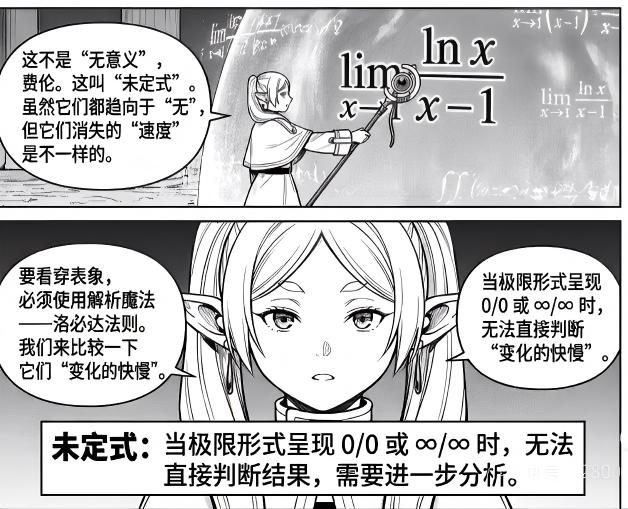
\includegraphics[width=0.7\linewidth]{figure/C6/222}
\end{center}
L'Hospital 法则用于处理函数极限的待定型$(\dfrac{\star}{\infty},\dfrac{0}{0})$
\begin{definition}
	(L'Hospital 法则)设 $f(x), g(x) \in D(a,a+d]$， $g'(x) \neq 0$.且下列条件之一成立：
	
	1.$\lim\limits_{x \to a^+} f(x) = \lim\limits_{x \to a^+} g(x) = 0$
	
	2.$	\lim\limits_{x \to a^+} g(x) = \pm \infty \text{ 或 } \infty$
	
	则有
	\[
	\lim_{x \to a^+} \frac{f(x)}{g(x)} = \lim_{x \to a^+} \frac{f'(x)}{g'(x)}
	\]
	
	
\end{definition}
注：此结论对以下极限行为均有效：
\[
x \to a^+, x \to a^-, x \to a, x \to \infty, x \to -\infty, x \to +\infty
\]

在相应的邻域内，有各自的洛必达法则成立.这里以 $x \to a^+$ 为例.
\begin{proof}
	先考虑 $\lim\limits_{x \to a^+} \dfrac{f'(x)}{g'(x)}$ 存在且有限的情况.设$\lim\limits_{x \to a^+} \dfrac{f'(x)}{g'(x)}=A$
	
	若满足情况1，令
	\[
	\ \widetilde{f}(x) = \begin{cases}
		0 & x = a, \\
		f(x) & x \in (a, a+d],
	\end{cases}
	\quad
	\widetilde{g}(x) = \begin{cases}
		0 & x = a, \\
		g(x) & x \in (a, a+d].
	\end{cases}
	\]
	
	$\widetilde{f}, \widetilde{g}\in C(a, a+d]$, 且对于 $x \in (a, a+d]$, $\widetilde{f}'(x) = f'(x)$, $\widetilde{g}'(x) = g'(x)$.
	
	由 $g'(x) \neq 0$ 及 Rolle 定理，$g(x)$ 在 $(a, a+d]$ 上至多有一个零点.
	必要时缩小 $d$，可设 $g(x) \neq 0$ 对一切 $x \in (a, a+d]$ 成立，从而 Cauchy 中值定理的条件满足.
	
	由 $\widetilde{f}(a) = \widetilde{g}(a) = 0$，对于 $x \in (a, a+d]$，
	\[
	\frac{f(x)}{g(x)} = \frac{\widetilde{f}(x) - \widetilde{f}(a)}{\widetilde{g}(x) - \widetilde{g}(a)}
	\]
	
	由 Cauchy 中值定理，$\exists \xi \in (a, x)$, 使得
	\[
	\frac{f(x)}{g(x)} = \frac{\widetilde{f}(x) - \widetilde{f}(a)}{\widetilde{g}(x) - \widetilde{g}(a)} = \frac{\widetilde{f}'(\xi)}{\widetilde{g}'(\xi)} = \frac{f'(\xi)}{g'(\xi)}
	\]
	
	当 $x \to a^+$ 时，$\xi \to a^+$，故
	\[
	\lim_{x \to a^+} \frac{f(x)}{g(x)} = \lim_{x \to a^+} \frac{f'(\xi)}{g'(\xi)}
	\]
	
	情况 2
	
	取 $x_0 \in(a, a+d]$ 且 $x_0$ 充分靠近 $a$ ．
	$$
	\begin{aligned}
		&\frac{f(x)}{g(x)}=\frac{f(x)-f\left(x_0\right)}{g(x)}+\frac{f\left(x_0\right)}{g(x)}=\frac{f(x)-f\left(x_0\right)}{g(x)-g\left(x_0\right)} \cdot \frac{g(x)-g\left(x_0\right)}{g(x)}+\frac{f\left(x_0\right)}{g(x)} \\
		&\frac{f(x)}{g(x)}-A=\left[\frac{f(x)-f\left(x_0\right)}{g(x)-g\left(x_0\right)}-A\right]\left(1-\frac{g\left(x_0\right)}{g(x)}\right)+A\left(1-\frac{g\left(x_0\right)}{g(x)}\right)+\frac{f\left(x_0\right)}{g(x)}-A \\
		&\left|\frac{f(x)}{g(x)}-A\right| \leqslant\left|\frac{f(x)-f\left(x_0\right)}{g(x)-g\left(x_0\right)}-A\right|\left|1-\frac{g\left(x_0\right)}{g(x)}\right|+\left|\frac{f\left(x_0\right)-A g\left(x_0\right)}{g(x)}\right|\quad(*)
	\end{aligned}
	$$
	
	$\exists \xi $介于$x, x_0$ 之间，使得
	\[
	\frac{f(x) - f(x_0)}{g(x) - g(x_0)} = \frac{f'(\xi)}{g'(\xi)}
	\]
	
	当 $x_0 \to a^+,x \to a^+$, $\xi \to a^+$, 由 $\lim\limits_{x \to a^+} \dfrac{f'(x)}{g'(x)} = A$，$\forall \varepsilon > 0$, $\exists \delta > 0$，当 $x \in (a, a+\delta)$ 时，
	\[
	\left|\frac{f'(x)}{g'(x)} - A\right| < \varepsilon
	\]
	
	取 $x \in (a, a+\delta)$，则 $\xi \in (a, a+\delta) \subset (a, a+d)$，
	\[
	\left|\frac{f'(\xi)}{g'(\xi)} - A\right| < \eps
	\]
	
	代入 $(*)$，
	\[
	\left|\frac{f(x)}{g(x)} - A\right| \leqslant 
	\eps \left|1 - \frac{g(x_0)}{g(x)}\right|+\left|\frac{f(x_0) - A g(x_0)}{g(x)}\right|
	\]
	
	对上述 $x_0$，
	\[
	\lim_{x \to a^+} \left(1 - \frac{g(x_0)}{g(x)}\right) = 1, \quad \lim_{x \to a^+} \frac{f(x_0) - A g(x_0)}{g(x)} = 0
	\]
	
	$\exists \rho$ 使得 $0 < \rho < \delta$，使得 $x \in (a, a+\rho)$ 时，
	\[
	\left|1 - \frac{g(x_0)}{g(x)}\right| < 1 + \frac{\eps}{2}, \quad \left|\frac{f(x_0) - A g(x_0)}{g(x)}\right| < \frac{\eps}{2}
	\]
	
	则
	\[
	\left|\frac{f(x)}{g(x)} - A\right| < \eps \left(1 + \frac{\eps}{2}\right) + \frac{\eps}{2}
	\]
	
	故
	\[
	\lim_{x \to a^+} \frac{f(x)}{g(x)} = A
	\]
	
	下面考虑 $\lim\limits_{x \to a^+} \dfrac{f'(x)}{g'(x)} = \pm\infty$ 的情况.从 $+\infty$ 为例.
	
	情况1: $\lim\limits_{x \to a^+} f(x) = \lim\limits_{x \to a^+} g(x) = 0$，考虑 $(a, a+d]$.
	
	令
	\[
	\ \widetilde{f}(x) = \begin{cases}
		0 & x = a, \\
		f(x) & x \in (a, a+d],
	\end{cases}
	\quad
	\widetilde{g}(x) = \begin{cases}
		0 & x = a, \\
		g(x) & x \in (a, a+d].
	\end{cases}
	\]
	
	由 $\lim\limits_{x \to a^+} \dfrac{f'(x)}{g'(x)} = +\infty$，$\forall G > 0$, $\exists \delta > 0$，$\forall x \in (a, a+\delta)$，使
	\[
	\frac{f'(x)}{g'(x)} > G
	\]
	
	由 Cauchy 中值定理，$\exists \xi \in (a, a+\delta)$ 使
	\[
	\frac{f(x)}{g(x)} = \frac{\widetilde{f}(x) - \widetilde{f}(a)}{\widetilde{g}(x) - \widetilde{g}(a)} = \frac{f'(\xi)}{g'(\xi)} > G
	\]
	
	故
	\[
	\lim_{x \to a^+} \frac{f(x)}{g(x)} = +\infty
	\]
	
	情况2: 设 $\lim\limits_{x \to a^+} g(x) = \infty$.任取 $x_0 \in (a, a+\delta)$, $\delta_1 \in (0, x_0 - a)$.使得当 $x \in (a, a+\delta_1)$ 时
	
	\[
	\max \left\{ \left|\dfrac{g(x_0)}{g(x)}\right|, \left|\dfrac{f(x_0)}{g(x)}\right|\right\} \leqslant \frac{1}{2}
	\]
	
	由
	\[
	\frac{f(x)}{g(x)} = \left[1 - \frac{g(x_0)}{g(x)}\right] \frac{f(x) - f(x_0)}{g(x) - g(x_0)} + \frac{f(x_0)}{g(x)}	= \left[1 - \frac{g(x_0)}{g(x)}\right] \frac{f'(\xi)}{g'(\xi)} + \frac{f(x_0)}{g(x)}
	\]
	对 $x \in (a, a+\delta_1)$ 时
	\[
	\left|\frac{f(x)}{g(x)}\right| \geqslant \frac{1}{2}(G + 1) - \frac{1}{2} = \frac{G}{2}
	\]
	
	故
	\[
	\lim_{x \to a^+} \frac{f(x)}{g(x)} = +\infty
	\]
	
\end{proof}

%
% 第8节：Taylor公式
% !TEX root = ../../../main.tex
% 所属：第一部分：单变量分析学 / 第7章：微分法
% 节：7.8 Taylor公式
% 正文按原文件顺序保存；由 ../chapter7.tex 调用。
\section{Taylor公式}
\begin{theorem}(带 Peano 余项的 Taylor 公式)
	设 $f(x)$ 在 $x = x_0$ 处有 $n$ 阶导数.则存在 $x_0$ 的邻域 $O(x_0, \delta)$，在 $O(x_0, \delta)$ 上，
	\[
	f(x) = f(x_0) + f'(x_0)(x-x_0) + \frac{1}{2!} f''(x_0)(x-x_0)^2 + \cdots + \frac{1}{n!} f^{(n)}(x_0)(x-x_0)^n + r_n(x)
	\]
	
	其中，$r_n(x) = o((x-x_0)^n)$，称为 Peano 余项.
	
	
\end{theorem}
\begin{proof}
	设
	\[
	r_n(x) = f(x) - \left[f(x_0) + f'(x_0)(x-x_0) + \cdots + \frac{1}{n!} f^{(n)}(x_0)(x-x_0)^n\right]
	\]
	下证 $r_n(x) = o((x-x_0)^n)$，也即
	\[
	\lim_{x \to x_0} \frac{r_n(x)}{(x-x_0)^n} = 0
	\]
	对 $n$ 用归纳法. $n=1$ 时，由导数的定义，
	\[
	f(x) = f(x_0) + f'(x_0)(x-x_0) + o(x-x_0),
	\]
	即 $r_1(x) = o(x-x_0)$，成立.
	
	假设结论对 $n$ 成立. 设 $f$ 在 $x_0$ 有 $n+1$ 阶导数，则 $f'$ 在 $x_0$ 有 $n$ 阶导数.
	将 $f$ 写成 $f(x)=P_{n+1}(x)+r_{n+1}(x)$，其中 $P_{n+1}$ 是 $n+1$ 次 Taylor 多项式.
	
	注意到 $r_{n+1}(x_0) = r_{n+1}'(x_0) = \cdots = r_{n+1}^{(n)}(x_0) = 0$，
	且 $r_{n+1}^{(n+1)}(x_0) = 0$. 反复应用 Cauchy 中值定理：
	\[
	\frac{r_{n+1}(x)}{(x-x_0)^{n+1}}
	= \frac{r_{n+1}'(\xi_1)}{(n+1)(\xi_1-x_0)^n}
	= \cdots
	= \frac{r_{n+1}^{(n)}(\xi_n)}{(n+1)!\,(\xi_n-x_0)},
	\]
	其中 $\xi_k$ 介于 $x_0$ 与 $\xi_{k-1}$ 之间（$\xi_0 = x$）.
	最后一步，
	\[
	\frac{r_{n+1}^{(n)}(\xi_n)}{\xi_n-x_0}
	= \frac{r_{n+1}^{(n)}(\xi_n) - r_{n+1}^{(n)}(x_0)}{\xi_n-x_0}
	\to r_{n+1}^{(n+1)}(x_0) = 0 \quad (\xi_n\to x_0).
	\]
	故 $r_{n+1}(x) = o((x-x_0)^{n+1})$，归纳完成.
\end{proof}
\begin{theorem}(带 Lagrange 余项的 Taylor 公式)
	设 $f(x) \in D^n[a, b]\cap D^{n+1}(a, b)$，任取 $ x_0 \in (a,b)$，$\exists \xi \in (a, b)$ 介于 $x$ 与 $x_0$ 之间，使得
	\[
	f(x) = f(x_0) + f'(x_0)(x-x_0) + \cdots + \frac{1}{n!} f^{(n)}(x_0)(x-x_0)^n + \frac{f^{(n+1)}(\xi)}{(n+1)!}(x-x_0)^{n+1}
	\]
	$r_n(x)=\dfrac{f^{(n+1)}(\xi)}{(n+1)!}(x-x_0)^{n+1}$称为Lagrange余项
\end{theorem}
\begin{proof}
	考虑辅助函数
	\[
	G(t) = f(x) - \sum_{k=0}^n \frac{1}{k!} f^{(k)}(t)(x-t)^k \quad \text{和} \quad H(t) = (x-t)^{n+1}.
	\]
	
	那么定理的结论（即需要证明的）是
	\[
	G(x_0) = \frac{f^{(n+1)}(\xi)}{(n+1)!} H(x_0).
	\]
	
	不妨设 $x_0 < x$（$x < x_0$ 时证明类似）.则 $G(t)$ 和 $H(t)$ 在 $[x_0, x]$ 上连续，在 $(x_0, x)$ 上可导，且
	
	\[\begin{aligned}
		G'(t) =& -[f'(t) + (-f'(t)) + f''(t)(x-t) + (-f''(t))(x-t)+ \frac{1}{2!} f'''(t)(x-t)^2 + \cdots\\&-\frac{1}{(n-1)!} f^{(n)}(t)(x-t)^{n-1} + \frac{f^{(n+1)}(t)}{n!}(x-t)^n]\\
		=&-\frac{1}{n!} f^{(n+1)}(t)(x-t)^n
	\end{aligned}\]
	
	\[
	H'(t) = -(n+1)(x-t)^n.
	\]
	
	显然 $H'(t)$ 在 $(x_0, x)$ 上不等于零.因为 $G(x) = H(x) = 0$，由 Cauchy 中值定理可得
	\[
	\frac{G(x_0)}{H(x_0)} = \frac{G(x) - G(x_0)}{H(x) - H(x_0)} = \frac{G'(\xi)}{H'(\xi)} = \frac{f^{(n+1)}(\xi)}{(n+1)!}, \quad \xi \in (x_0, x),
	\]
	
	由此 $G(x_0) = \dfrac{f^{(n+1)}(\xi)}{(n+1)!} H(x_0)$.
\end{proof}
\begin{corollary}(Maclaurin 公式)
	在 $x_0=0$ 时的 Taylor 公式，即为 Maclaurin 公式，
	$$
	f(x) = f(0) + f'(0)x + \frac{1}{2!} f''(0)x^2 + \cdots + \frac{1}{n!} f^{(n)}(0)x^n + r_n(x)
	$$
	
	其中余项
	$$
	r_n(x) = o(x^n) \quad \text{或} \quad \frac{f^{(n+1)}(\xi)}{(n+1)!} x^{n+1} \quad (\xi \text{ 介于 } 0 \text{ 与 } x \text{ 之间})
	$$
\end{corollary}
利用上面的公式，代入一些函数，可以直接得到以下函数的Maclaurin展开
\begin{proposition}
	在$x=0$的邻域内，有
	
	1.
	\[
	e^x = 1 + x + \frac{1}{2!}x^2 + \frac{1}{3!}x^3 + \cdots + \frac{1}{n!}x^n + r_n(x)
	\]
	
	推论：
	\[
	\lim_{n \to \infty} \left(1 + 1 + \frac{1}{2!} + \cdots + \frac{1}{n!}\right) = e
	\]
	
	2.
	\[
	\cos x = 1 - \frac{1}{2!}x^2 + \frac{1}{4!}x^4 - \frac{1}{6!}x^6 + \cdots + \frac{(-1)^n}{(2n)!}x^{2n} + r_{2n+1}(x)
	\]
	
	\[
	\sin x = x - \frac{1}{3!}x^3 + \frac{1}{5!}x^5 - \frac{1}{7!}x^7 + \cdots + \frac{(-1)^n}{(2n+1)!}x^{2n+1} + r_{2n+2}(x)
	\]
	
	\[
	\tan x = x + \frac{1}{3}x^3 + \frac{2}{15}x^5 + \frac{17}{315}x^7 + r_9(x)
	\]
	
	3. 对于 $f(x) = (1+x)^\alpha$, $\alpha \in \mathbb{R}$,
	
	\[\begin{aligned}
		f(x) &= (1+x)^\alpha = 1 + C_\alpha^1 x + C_\alpha^2 x^2 + \cdots + C_\alpha^{\alpha-1} x^{\alpha-1} + x^\alpha\\
		&\Rightarrow C_\alpha^0 + C_\alpha^1 x + \cdots + C_\alpha^n x^n + r_n(x) \quad (n < \alpha \text{ 时})\\
		&\Rightarrow C_\alpha^0 + C_\alpha^1 x + \cdots + C_\alpha^{\alpha-1} x^{\alpha-1} + x^\alpha \quad (n > \alpha \text{ 时})
	\end{aligned}	\]
	
	
	若$ \alpha \notin \mathbb{Z}_+$, $\forall k \in \mathbb{R}$, $C_\alpha^k \neq 0$,
	\[
	(1+x)^\alpha = 1 + \alpha x + \frac{\alpha(\alpha-1)}{2!}x^2 + \cdots + \frac{\alpha(\alpha-1)\cdots(\alpha-n+1)}{n!}x^n + r_n(x)
	\]
	
	当 $\alpha = -1$ 时，
	\[
	\frac{1}{1+x} = 1 - x + x^2 - x^3 + x^4 - \cdots + (-1)^n x^n + r_n(x)\quad(*)
	\]
	
	对于 $\alpha = \dfrac{1}{2}$，
	\[
	\sqrt{1+x} = 1 + \frac{1}{2}x - \frac{1}{2 \cdot 4}x^2 + \frac{1 \cdot 3}{2 \cdot 4 \cdot 6}x^3 - \cdots + (-1)^{n-1} \frac{(2n-3)!!}{(2n)!!}x^n + r_n(x)
	\]
	
	系数为
	\[
	\begin{cases}
		\dfrac{1}{2} & \text{当 } k=1, \\
		(-1)^{k-1} \dfrac{(2k-3)!!}{(2k)!!} & \text{当 } k > 1.
	\end{cases}
	\]
	
	对于 $\alpha = -\dfrac{1}{2}$，
	\[
	\frac{1}{\sqrt{1+x}} = 1 - \frac{1}{2}x + \frac{1 \cdot 3}{2 \cdot 4}x^2 - \frac{1 \cdot 3 \cdot 5}{2 \cdot 4 \cdot 6}x^3 + \cdots + (-1)^n \frac{(2n-1)!!}{(2n)!!}x^n + r_n(x)
	\]
	
	系数为
	\[
	(-1)^n \frac{(2n-1)!!}{(2n)!!}.
	\]
	
	对于 $(*)$，分别代入$-x,x^2,-x^2$：
	\[
	\frac{1}{1-x} = 1 + x + x^2 + x^3 + \cdots + x^n + r_n(x)
	\]
	\[
	\frac{1}{1+x^2} = 1 - x^2 + x^4 - x^6 + \cdots + (-1)^n x^{2n} + r_{2n}(x)
	\]
	\[
	\frac{1}{1-x^2} = 1 + x^2 + x^4 + \cdots + x^{2n} + r_{2n}(x)
	\]
\end{proposition}
这里介绍一条定理，用于计算一些函数的展开
\begin{proposition}
	在$x_0$的某个邻域内，$f(x)\in D^{n+2}$，则它的$n+1$次Taylor多项式的导数恰为$f'(x)$的$n$次Taylor 展开
\end{proposition}
\begin{proof}
	设
	\[
	f(x) = f(x_0) + f'(x_0)(x-x_0) + \cdots + \frac{1}{(n+1)!} f^{(n+1)}(x_0)(x-x_0)^{n+1} + r_{n+1}(x)
	\]
	
	\[
	f'(x) = P_{n+1}(x) = f'(x_0) + f''(x_0)(x-x_0) + \cdots + \frac{1}{n!} f^{(n)}(x_0)(x-x_0)^n + r'_{n+1}(x)
	\]
	
	这意味着存在 $g_n(x)$ 使得
	\[
	\lim_{x \to x_0} \frac{r'_{n+1}(x)}{g_n(x)} = 1
	\]
	
	\[
	f'(x) = f'(x_0) + f''(x_0)(x-x_0) + \cdots + \frac{1}{n!} f^{(n)}(x_0)(x-x_0)^n + g_n(x)
	\]
	
	且
	\[
	\lim_{x \to x_0} g_n(x) = 0
	\]
\end{proof}
\begin{proposition}
	1. 已知
	\[
	\frac{1}{1+x} = 1 - x + x^2 - x^3 + \cdots + (-1)^n x^n + r_n(x)
	\]
	
	设
	\[
	\ln(1+x) = a_0 + a_1 x + \cdots + a_n x^n + r_n(x)
	\]
	
	对 $\ln(1+x)$ 求导，
	\[\begin{aligned}
		(\ln(1+x))' &= a_1 + 2a_2 x + \cdots + n a_n x^{n-1} + r_{n-1}(x)\\&= \frac{1}{1+x} = 1 - x + x^2 - \cdots + (-1)^n x^n + r_{n-1}(x)
	\end{aligned}\]
	得
	\[
	\ln(1+x) = x - \frac{1}{2}x^2 + \frac{1}{3}x^3 - \cdots + (-1)^{n-1} \frac{1}{n} x^n + r_n(x)
	\]
	
	同理
	\[
	\ln(1-x) = -x - \frac{1}{2}x^2 - \frac{1}{3}x^3 - \cdots - \frac{1}{n}x^n + r_n(x)
	\]
	2. 由 $(\tan^{-1} x)' = \dfrac{1}{1+x^2} = 1 - x^2 + x^4 - x^6 + \cdots + (-1)^n x^{2n} + r_{2n}(x)$，
	得
	\[
	\tan^{-1} x = x - \frac{1}{3}x^3 + \frac{1}{5}x^5 - \frac{1}{7}x^7 + \cdots + (-1)^n \frac{1}{2n+1} x^{2n+1} + r_{2n+1}(x)
	\]
	
	类似地，
	\[
	\sin^{-1} x = x + \frac{1}{2} \cdot \frac{1}{3} x^3 + \frac{1 \cdot 3}{2 \cdot 4} \cdot \frac{1}{5} x^5 + \cdots + \frac{(2n-1)!!}{(2n)!!} \cdot \frac{1}{2n+1} x^{2n+1} + r_{2n}(x)
	\]
	
	而
	\[
	\cos^{-1} x = \frac{\pi}{2} - \sin^{-1} x
	\]
	
	3. 对于 $a^x = e^{x \ln a}$，
	\[
	a^x = 1 + x \ln a + \frac{1}{2!} (x \ln a)^2 + \cdots + \frac{1}{n!} (x \ln a)^n + r_n(x)
	\]
	
	4.
	\[
	\ln \left(\frac{1+x}{1-x}\right) = 2 \left(x + \frac{1}{3}x^3 + \cdots + \frac{1}{2n+1}x^{2n+1}\right) + r_{2n+1}(x)
	\]
	
	5.
	\[
	\cosh x = 1 + \frac{1}{2!}x^2 + \frac{1}{4!}x^4 + \cdots + \frac{1}{(2n)!}x^{2n} + r_{2n}(x)
	\]
	
	\[
	\sinh x = x + \frac{1}{3!}x^3 + \frac{1}{5!}x^5 + \cdots + \frac{1}{(2n-1)!}x^{2n-1} + r_{2n-1}(x)
	\]
\end{proposition}

%
% 第9节：一些应用
% !TEX root = ../../../main.tex
% 所属：第一部分：单变量分析学 / 第7章：微分法
% 节：7.9 一些应用
% 正文按原文件顺序保存；由 ../chapter7.tex 调用。
\section{一些应用}
\begin{definition}
	函数 $f(x)$ 在无穷区间有定义，若 $f(x)$ 的斜近线为 $y = ax + b$，则满足
	\[
	\lim_{x \to +\infty} \left[ f(x) - (ax + b) \right] = 0
	\]
	
	易知
	\[
	\lim_{x \to +\infty} \frac{f(x)}{x} = a, \quad \lim_{x \to +\infty} \left[ f(x) - ax \right] = b
	\]
	
	水平渐近线是斜渐近线 $a=0$ 时的退化形式
	
	垂直渐近线是 $x=a$.满足
	\[
	\lim_{x \to a} f(x) = +\infty, -\infty \text{ 或 } \infty
	\]
	
	此处可 $x \to a$，$x \to a^+$，$x \to a^-$.
\end{definition}
另外一种应用是

\textbf{极值点的判定}
	
	函数 $f(x)$ 在区间 $(a, b)$ 上有定义，有以下两种情况：
	
	1. $f(x)$ 在 $x_0$ 处不可导：用极值点定义判别.
	
	2. $f(x)$ 在 $x_0$ 处可导，且 $f'(x_0) = 0$，进一步判别：
	
	若存在 $\delta > 0$，使得 $f(x)$ 在区间 $(x_0 - \delta, x_0 + \delta)$ 内有定义（否则使用极值点的定义）：
	
	(1) 二阶导数不存在：
	
	(i) $\forall x \in (x_0 - \delta, x_0), f'(x)\geqslant0$ 且 $\forall x \in (x_0, x_0 + \delta), f'(x)\leqslant0$ 时，$x_0$ 是极大值点
	
	(ii) $\forall x \in (x_0 - \delta, x_0), f'(x)\leqslant0$ 且 $\forall x \in (x_0, x_0 + \delta), f'(x)\geqslant0$ 时，$x_0$ 是极小值点
	
	(iii) $(x_0 - \delta,x_0),(x_0, x_0 + \delta)$ 上$f'(x)$同号，则不存在极值点
	
	(2) 二阶导数存在：
	
	在 $(x_0 - \delta, x_0 + \delta)$ 内，
	\[ f(x) = f(x_0) + f'(x_0)(x-x_0) + \frac{1}{2!} f''(x_0)(x-x_0)^2 \]
	
	\[ f(x) - f(x_0) = \frac{1}{2!} f''(x_0)(x-x_0)^2 \]
	
	当 $f''(x_0) > 0$ 时，$x_0$ 为严格极小值点，
	
	当 $f''(x_0) < 0$ 时，$x_0$ 为严格极大值点.

\subsection*{绘制图像的一般步骤}

导数为我们提供了系统绘制函数图像的工具。借助一阶导数和二阶导数，我们可以确定函数的单调区间、极值点、凹凸性、拐点，并结合渐近线等信息，勾勒出函数的大致图像。



绘制函数 $y=f(x)$ 图像的步骤如下：

\begin{enumerate}
	\item \textbf{确定定义域}：找出 $f(x)$ 的自然定义域，并关注间断点。
	\item \textbf{奇偶性与周期性}：判断 $f(x)$ 是否具有奇偶性或周期性，可简化后续分析。
	\item \textbf{一阶导数 $f'(x)$}：求出 $f'(x)$ 及其零点（驻点）和不存在点，利用 $f'(x)$ 的符号划分单调区间，并用第一或第二充分条件判定极值。
	\item \textbf{二阶导数 $f''(x)$}：求出 $f''(x)$ 及其零点和不存在点，确定凹凸区间与拐点。
	\item \textbf{渐近线}：计算水平渐近线、垂直渐近线和斜渐近线。
	\item \textbf{关键点与辅助点}：计算驻点、拐点、与坐标轴的交点等关键位置的函数值，必要时补充若干辅助点。
	\item \textbf{描点连线}：在坐标系中标出所有关键点，结合单调性、凹凸性和渐近线，平滑地连接成函数图像。
\end{enumerate}



\begin{example}
	绘制函数 $f(x)=\dfrac{x^3}{x^2-1}$ 的图像。
\end{example}

\begin{proof}[解]
	\textbf{1. 定义域}：分母 $x^2-1\neq0$，故定义域为 $(-\infty,-1)\cup(-1,1)\cup(1,+\infty)$。

	\textbf{2. 奇偶性}：
	\[
	f(-x)=\frac{(-x)^3}{(-x)^2-1}=-\frac{x^3}{x^2-1}=-f(x)
	\]
	$f(x)$ 为奇函数，图像关于原点对称。

	\textbf{3. 一阶导数}：
	\[
	f'(x)=\frac{3x^2(x^2-1)-x^3\cdot 2x}{(x^2-1)^2}=\frac{x^2(x^2-3)}{(x^2-1)^2}
	\]
	令 $f'(x)=0$，得 $x=0$，$x=\pm\sqrt{3}$。

	单调性分析：

	\begin{center}
		\begin{tabular}{c|ccccccccc}
			$x$ & $(-\infty,-\sqrt{3})$ & $-\sqrt{3}$ & $(-\sqrt{3},-1)$ & $(-1,0)$ & $0$ & $(0,1)$ & $(1,\sqrt{3})$ & $\sqrt{3}$ & $(\sqrt{3},+\infty)$ \\
			\hline
			$f'(x)$ & $+$ & $0$ & $-$ & $-$ & $0$ & $-$ & $-$ & $0$ & $+$ \\
			$f(x)$ & $\nearrow$ & 极大 & $\searrow$ & $\searrow$ & 拐点 & $\searrow$ & $\searrow$ & 极小 & $\nearrow$
		\end{tabular}
	\end{center}

	极大值 $f(-\sqrt{3})=-\dfrac{3\sqrt{3}}{2}$，极小值 $f(\sqrt{3})=\dfrac{3\sqrt{3}}{2}$。

	\textbf{4. 二阶导数}：
	\[
	f''(x)=\frac{2x(x^2+3)}{(x^2-1)^3}
	\]
	令 $f''(x)=0$，得 $x=0$。

	凹凸性分析：

	\begin{center}
		\begin{tabular}{c|ccccc}
			$x$ & $(-\infty,-1)$ & $(-1,0)$ & $0$ & $(0,1)$ & $(1,+\infty)$ \\
			\hline
			$f''(x)$ & $-$ & $+$ & $0$ & $-$ & $+$ \\
			$f(x)$ & 上凸 & 下凸 & 拐点 & 上凸 & 下凸
		\end{tabular}
	\end{center}

	拐点 $(0,0)$。

	\textbf{5. 渐近线}：
	\[
	\lim_{x\to\pm 1^{\mp}}f(x)=\infty,\quad \lim_{x\to\pm 1^{\pm}}f(x)=\mp\infty
	\]
	$x=-1$ 和 $x=1$ 为垂直渐近线。

	\[
	a=\lim_{x\to\infty}\frac{f(x)}{x}=\lim_{x\to\infty}\frac{x^2}{x^2-1}=1
	\]
	\[
	b=\lim_{x\to\infty}[f(x)-ax]=\lim_{x\to\infty}\frac{x}{x^2-1}=0
	\]
	$y=x$ 为斜渐近线（当 $x\to+\infty$ 和 $x\to-\infty$ 时均成立）。

	\textbf{6. 辅助点}：
	\[
	f(0)=0,\quad f\left(\pm\frac{1}{2}\right)=\mp\frac{1}{6},\quad f(\pm 2)=\pm\frac{8}{3}
	\]

	\textbf{7. 绘制图像}：综合以上信息，先画出三条渐近线 $x=-1$、$x=1$ 和 $y=x$，再标出极值点与拐点，最后按照单调性和凹凸性平滑连接即可。
\end{proof}

上述例子展示了利用导数绘制函数图像的一般流程。在更复杂的情形中，若函数含有指数、对数或三角函数，仍需遵循相同的分析框架，逐项确定定义域、单调性、凹凸性和渐近线，最后综合成图。
%
